\documentclass{article}

\usepackage{../preamble/factory, ../preamble/font, ../preamble/math, ../preamble/math_font, ../preamble/style, ../preamble/theorem}

\newtheorem{thr}{Uppgift}

\begin{document}

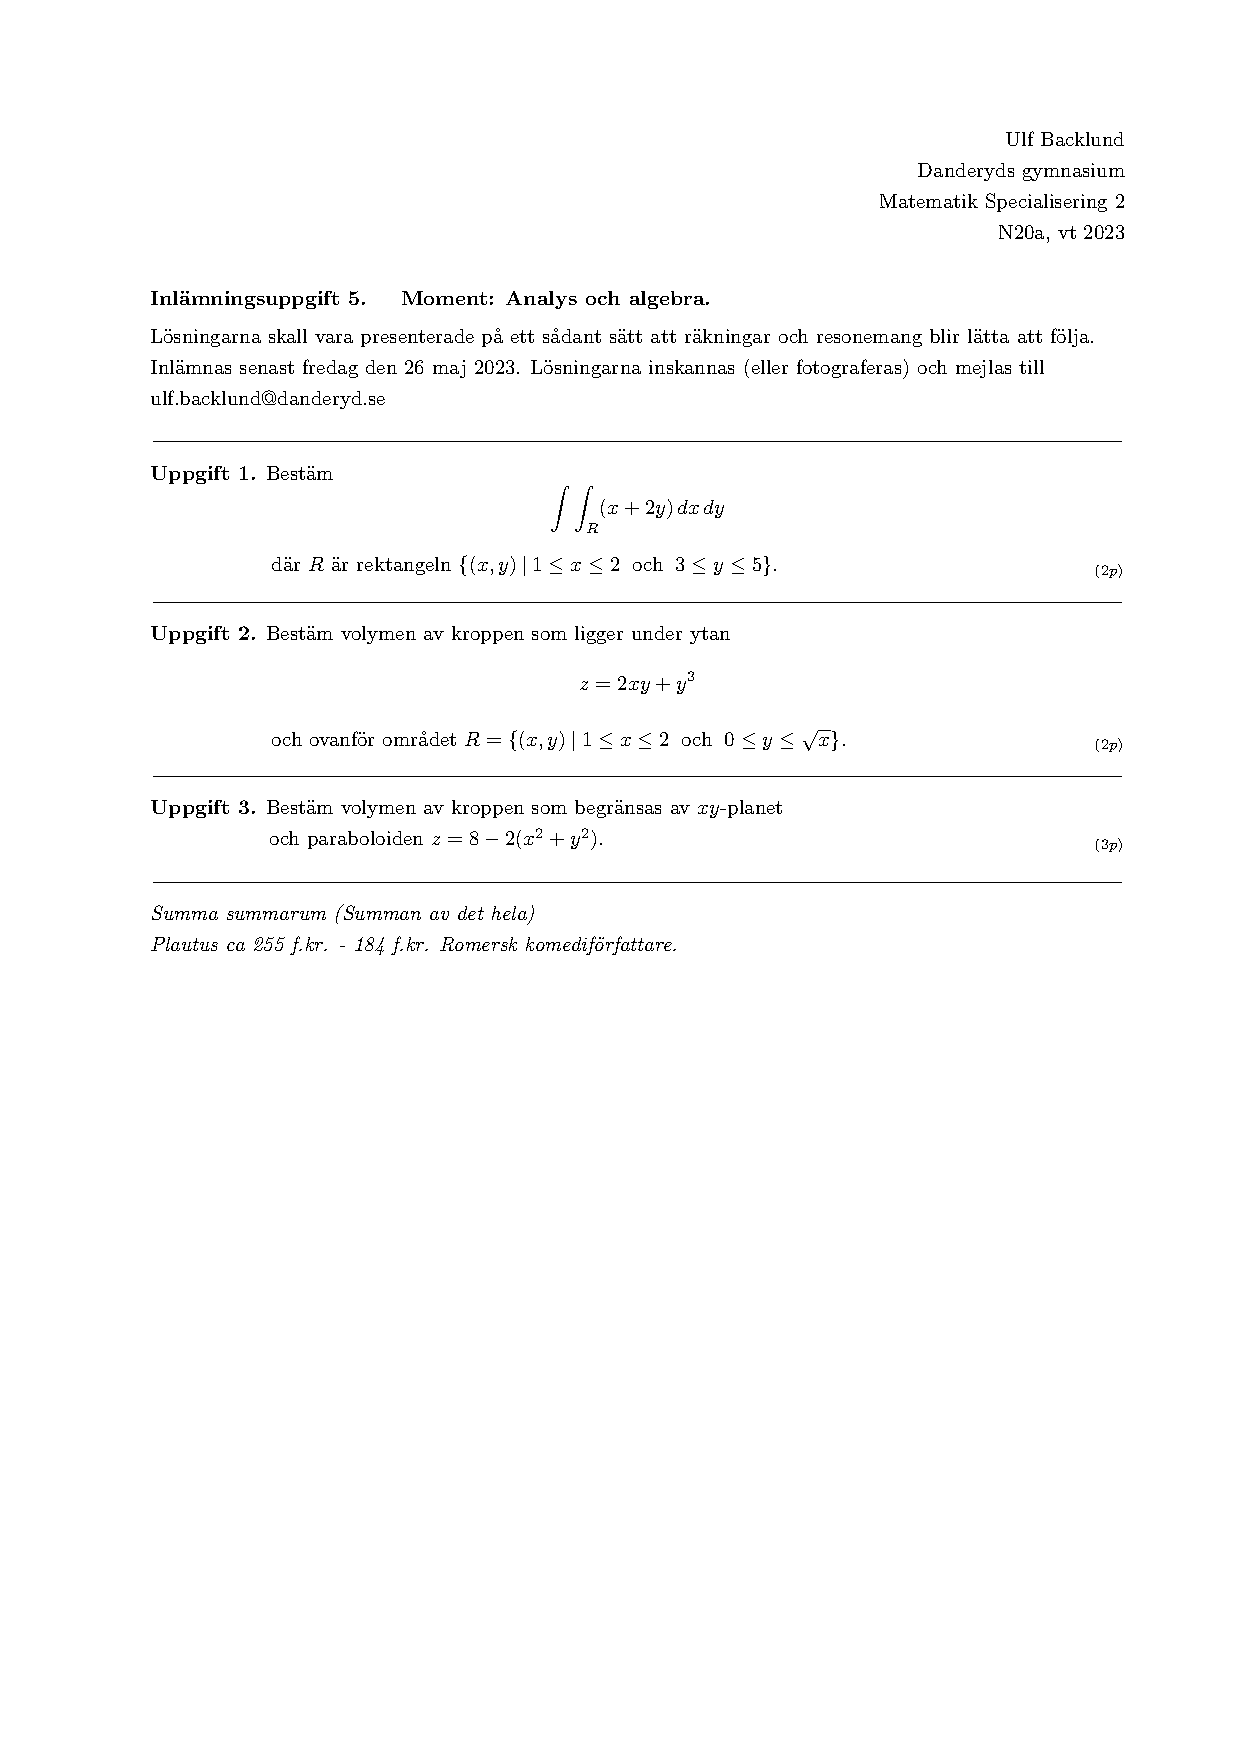
\includepdf{homework_5}

\newpage

\centerline{\large Matematik specialisering 2 inlämning 5}

\vskip 0.1cm

\centerline{\scriptsize Adam Amanbaev}

\begin{thr}
\end{thr}

$$
\therefore\;
R=\{(x, y) \build 1\leq x\leq2 \Och 3\leq y\leq5\}
$$

$$
\iint_{R}(x+2y)\:dx\:dy
=
\int_{3}^{5}\int_{1}^{2}((x+2y)\:dx)\:dy
\;\;\text{\scriptsize (Fubini's sats)}
$$

$$
=
\int_{3}^{5}\left[\frac{x^2}{2}+2yx\right]_{1}^{2}\;dy
=
\int_{3}^{5}2+4y-\frac{1}{2}-2y\;dy
=
\int_{3}^{5}\frac{3}{2}+2y\;dy
$$

$$
=
\left[y^2+\frac{3}{2}y\right]_{3}^{5}
=
5^2+5*\frac{3}{2}-3^2-3*\frac{3}{2}
=
19 
$$

\newpage

\begin{thr}
\end{thr}

$$
\therefore\;
R=\{(x, y) \build 1\leq x\leq2 \Och 0\leq y \leq \sqrt{x}\} \Och z=2xy+y^3
$$

\vskip 0.5cm

Området $R$ är y-enkelt vilket gör att volymen, $V$, av kroppen under ytan $z$ kan beskrivas av följande dubbelintegral:

$$
V=
\int_{1}^{2}\int_{0}^{\sqrt{x}}((2xy+y^3)\;dy)\;dx 
=
\int_{1}^{2}\left[xy^2+\frac{y^4}{4}\right]_{0}^{\sqrt{x}}\;dx\;\;\text{\scriptsize (Fubini's sats)}
$$

$$
=
\int_{1}^{2}x^2+\frac{x^2}{4}-0 \; dx
=
\frac{5}{4}\int_{1}^{2}x^2 \; dx
=
\frac{5}{4}\left[\frac{x^3}{3}\right]_{1}^{2}
=
\frac{5}{4}(\frac{2^3}{3}-\frac{1^3}{3})
$$

$$
=
\frac{5}{4}(\frac{7}{3})
=
\frac{35}{12} \; \text{v.e}
$$

$$
\therefore \; \text{Volymen av kroppen över $R$ och under ytan $z$ är lika med}\; V=\frac{35}{12} \;\text{v.e}.
$$

\newpage

\begin{thr}
\end{thr}

Vi studerar först området, $R$, på $xy$-planet som volymen är över. Det är området då $z=0$:

$$
z=0 
\Imp 
8-2(x^2+y^2)=0
\Imp
x^2+y^2=2^2
$$

$$
\Imp
R=\{(x, y) \build x^2+y^2=2^2\}
$$

\vskip 0.2cm

Området $R$ är alltså en cirkel med radie 2 och centrum i $(0, 0)$. Volymen, $V$, av kroppen som begränsas av området $R$ i $xy$-planet och paraboloiden $z=8-2(x^2+y^2)$ kan beskrivas av följande dubbelintegral:

\vskip 0.1cm

$$
V=
\iint_{R} z \;dA=
\iint_{R} 8-2(x^2+y^2) \;dA=_{\;\text{\scriptsize polära koordinater}}
$$

$$
=
\int_{0}^{2\pi}\int_{0}^{2}((8-2r^2)r\;dr)\;d\theta \;\;\;\text{\scriptsize(jacobianen $r$)}
$$

$$
=
\int_{0}^{2\pi}\int_{0}^{2}(8r-2r^3\;dr)\;d\theta \;\;\;
=
\int_{0}^{2\pi}\left[4r^2-\frac{r^4}{2}\right]_{0}^{2}\;d\theta
$$

$$
=
\int_{0}^{2\pi}4*2^2-\frac{2^4}{2}-4*0^2+\frac{0^4}{2} \;d\theta
=
$$

$$
=
\int_{0}^{2\pi}8 \;d\theta
=
\left[8\theta\right]_{0}^{2\pi}
=
8*2\pi-8*0
=
16\pi \;\text{v.e}
$$

$$
\therefore\;\text{Volymen av kroppen som begränsas av $xy$-planet och $z$ är lika med}\; V=16\pi\;\text{v.e}.
$$

\end{document}
